% !TEX encoding = UTF-8 Unicode

\Chapter{Matematikai eszközök}

\Section{Zaj szűréshez, elmosáshoz használatos szűrők}

A következő szakaszokban annak bemutatására kerül majd sor, hogy a tervezett művészi szűrők létrehozásához milyen matematikai apparátusra van szükség. Ez alapvetően a különféle szűrési eljárások megvalósítását takarja példákkal illusztrálva.

A módszerek digitális képfeldolgozás területén közismertnek tekinthetők. A témakör feldolgozásához Kató Zoltán \textit{Digitális képfeldolgozás} című kurzusának anyagai szolgáltak alapul \cite{kato}.

\SubSection{Átlagoló szűrő}

Az átlagoló szűrő segítségével simítani lehet a képet. A képpontok közelebb kerülnek a környezetük átlagához, azaz a kép "simább" lesz, a szűrt kép intenzitásértékei a kiinulási kép intenzitástartományában maradnak. Csökkenti a zajt, de elmossa az éleket igy homályossá teszi a képet.

\example{Itt látható a átlagoló szűrésre egy példa, egy képpont 3x3 as környezete:
$$
\frac{1}{9} \times
\begin{bmatrix}
54 &26  &32 \\ 
17 &36  &24 \\ 
11 &23  &47 
\end{bmatrix}.
$$
Egyszerű simítási technika, ahol az ablakban lévő intenzitások átlaga az új intenzitás érték: 
$$
\bar{x} =
\frac{54+26+32+17+36+24+11+23+47}{9} =
\frac{270}{9} = 30.
$$}

%http://www.tankonyvtar.hu/en/tartalom/tamop412A/2011-0063_15_gepi_latas/ch05s02.html
%Kató tanár úr jegyzet
%wikipédia

\SubSection{Gauss szűrő}

A Gauss szűrő egy bemeneti kép és egy Gauss-kernel konvoluciójával jön létre. Minden egyes képpont értéket a környékének súlyozott átlagaként számolunk úgy, hogy a képpont eredeti értékének a legnagyobb a súlya, míg a távoliak kisebb súlyt kapnak. Ez olyan elmosódást eredményez, amely jobban védi a széleket, mint más egyenletes elmosódási algoritmusok. Egy Gauss függvény egyenlete egy dimenzióban az alábbi
$$
G(x) =
\frac{1}{\sqrt{2\pi\sigma^{2}}}
\cdot e^{-\frac{x^{2}}{2\sigma^{2}}}.
$$

A Gauss függvény grafikonját \aref{fig:gauss}. ábrán láthatjuk.

% 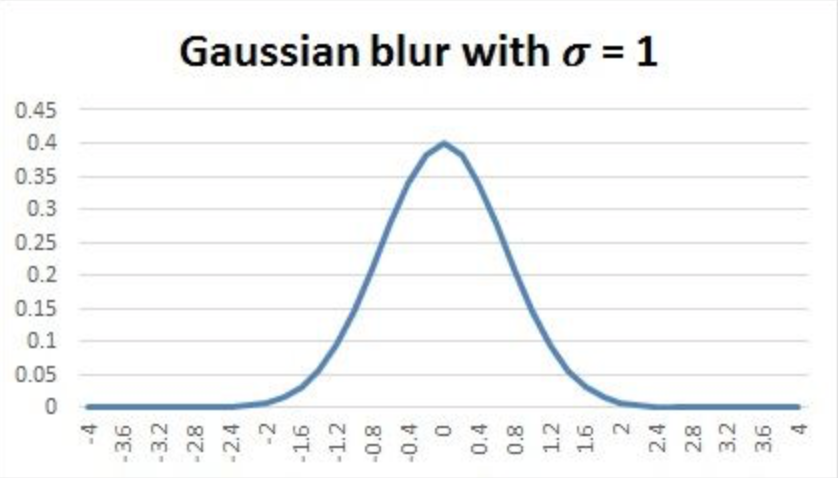
\epsfig{file=kepek/gaussgorbe.png,scale=0.65}

\begin{figure}[h!]
% \centering
\begin{tikzpicture}
\begin{axis}[every axis plot post/.append style={
  mark=none,domain=-4:4,samples=50,smooth},
  axis x line=bottom,
  axis y line=left,
  enlargelimits=upper]
  \addplot {gauss(0, 1)};
\end{axis}
\end{tikzpicture}
\caption{Az egydimenziós Gauss függvény $\mu = 0$ és $\sigma = 1$ paraméterekkel}
\label{fig:gauss}
\end{figure}

Két dimenzióban, két Gauss együttesét kell használni, minden egyes dimenzióban: 
$$
G(x,y) =
\frac{1}{\sqrt{2\pi\sigma^{2}}} \cdot
e^{-\frac{x^{2}+y^{2}}{2\sigma^{2}}},
$$
ahol az $x$ a vízszintes tengely eredetétől való távolság, az $y$ a függőleges tengely eredetétől való távolság, a $\sigma$ pedig a Gauss eloszlás szórása. Két dimenzióban alkalmazva, ez a képlet olyan felületet hoz létre, amelynek körvonalait koncentrikus körök alkotják, a Gauss-eloszlás pedig a középpontból indul.
%wikipédia
%Kató tanár úr jegyzet
%http://fiveko.com/tutorials/image-processing/gaussian-blur-filter/

\SubSection{Medián szűrő}

Az $a_1, a_2, \dots, a_{2n+1} \in \mathbb{R}$ számok mediánja, a nagyság szerint rendezett számsorozat középső, $(n+1)$-edik eleme. Jelölhetjük például a
$med\{a_1,a_2,\dots,a_{2n+1}\}$ formában.

Teljesül rá az alábbiak:
\begin{itemize}
\item $\min\{a_i\} \leq med\{a_i\} \leq \max\{a_i\}$,
\item $\min\{a_i+c\} = med\{a_i\}+c$,
\item $med\{c\cdot a_i\}=c \cdot med\{a_i\}$.
\end{itemize}

A medián szűrést egy $S \in \mathbb{R}^2$ környezet felett a
$$
J(i,j) = med\left\{I(i+u, j+v) \mid (u, v) \in S \right\}
$$
formában végezhetjük el.

A medián szűrés eredményét az $S$ környezet mérete (és alakja) határozza meg.

\example{Itt látható a medián szűrésre egy példa, egy képpont $3 \times 3$ méretű környezete: $$
\begin{bmatrix}
54 &25  &32 \\ 
17 &37  &22 \\ 
11 &23  &45 
\end{bmatrix}.$$
Nagyság szerint sorba rendezve ezeket az értékeket, úgy hogy  11, 17, 22, 23, 25, 32, 37, 45, 54 akkor a pixel új intenzitása 25 lesz, mivel az a középső érték a sorban.}

%Kató tanár úr jegyzet
\SubSection{Kétoldalú szűrő}

A kétoldalaú szűrő egy nem lineáris, élvédő és zajcsökkentő simító szűrő a képekhez \cite{bilateral}. Az egyes képpontok intenzitását a közeli pixelek intenzitásának súlyozott átlagával helyettesíti. Ez a súly Gauss eloszláson is  alapulhat. Elengedhetetlen, hogy a súlyok nem csak az euklideszi képpontok távolságától, hanem a radiometriai különbségektől is függnek (például tartománykülönbségek, például színintenzitás, mélységi távolság stb.). Ez a kép éles széleit megőrzi. A kétoldalú-szűrő az alábbi alakban írható föl:
\begin{align*}
I^{filtered}(x) &=
\frac{1}{W_p}\sum_{x_i\in\Omega}{I(x_i)f_r(\left \| I(x_i)-I(x) \right \|)g_s(\left \| x_i-x \right \|)}, \\
W_p &=
\sum_{x_i \in \Omega} f_r(\left \| I(x_i)-I(x) \right \|)g_s(\left \| x_i-x \right \|),
\end{align*}
ahol
\begin{itemize}
\item $I^{filtered}$ a filterrel ellátott kép,
\item $I$ az eredeti bemeneti kép,
\item $x$ a koorditánái a jelenlegi pixeleknek amik a szűrőbe kerülnek,
\item $\omega$ az ablak közepe $x$-nek,
\item $f_r$ a tartományi kernel az intenzitások közötti különbségek simítására,
\item $g_s$ a térbeli kernel a koordináták közötti különbségek simítására.
\end{itemize}
A $W_p$ súlyt a térbeli közelség és az intenzitás különbség alkalmazásával határoztuk meg. Vegyünk egy pixelt az $(i, j)$ koordinátákon, amelyet a szomszédos képpontok segítségével kell zajcsökkenteni a képen, és az egyik szomszédos pixele a $(k, l)$ helyen található. Ezután a pixelhez $(k, l)$ hozzárendelt súly az $(i, j)$ pixel zajcsökkentéséhez a következőket adja meg:
$$
w(i, j, k, l) =
\exp \left(
-\frac{(i-k)^{2}+(j-l)^{2}}{2\sigma_{s}^{2}}
-\frac{\left \| I(i,j)-I(k,l) \right \|^{2}}{2\sigma_{r}^{2}}
\right),
$$
ahol $\sigma_s$ és $\sigma_r$ a kiegyenlítési paraméterek, és $I(i, j)$ és $I(k, l)$ a pixelek $(i, j)$ és $(k, l)$ intenzitása.

A súlyok kiszámítása után normalizáljuk őket:
$$
I_{D}(i,j) =
\frac{\sum_{k,l}I(k,l)w(i, j, k, l)}{\sum_{k, l}w(i, j, k, l)},
$$
ahol az $I_D$ a pixel $(i, j)$ zajcsökkentés intenzitása.

A kétoldalú szűrőt két paraméterrel lehet irányítani: $\sigma_r$ és $\sigma_s$. Ezen paraméterek hatását \aref{fig:bilateral}. ábrán láthatjuk.
\begin{itemize}
\item Amikor a $\sigma_r$ paraméter növekszik, a kétoldalas szűrő fokozatosan megközelíti a Gauss konvolúciót, mivel a Gauss-tartomány kiszélesedik és kilapul, ami azt jelenti, hogy a kép intenzitási intervalluma alatt majdnem állandóvá válik.
\item Ahogy a $\sigma_s$ térbeli paraméter nő, a hozzá tartozó nagyobb értékek szerint a kép simább lesz.
\end{itemize}

\begin{figure}[h!]
\centering
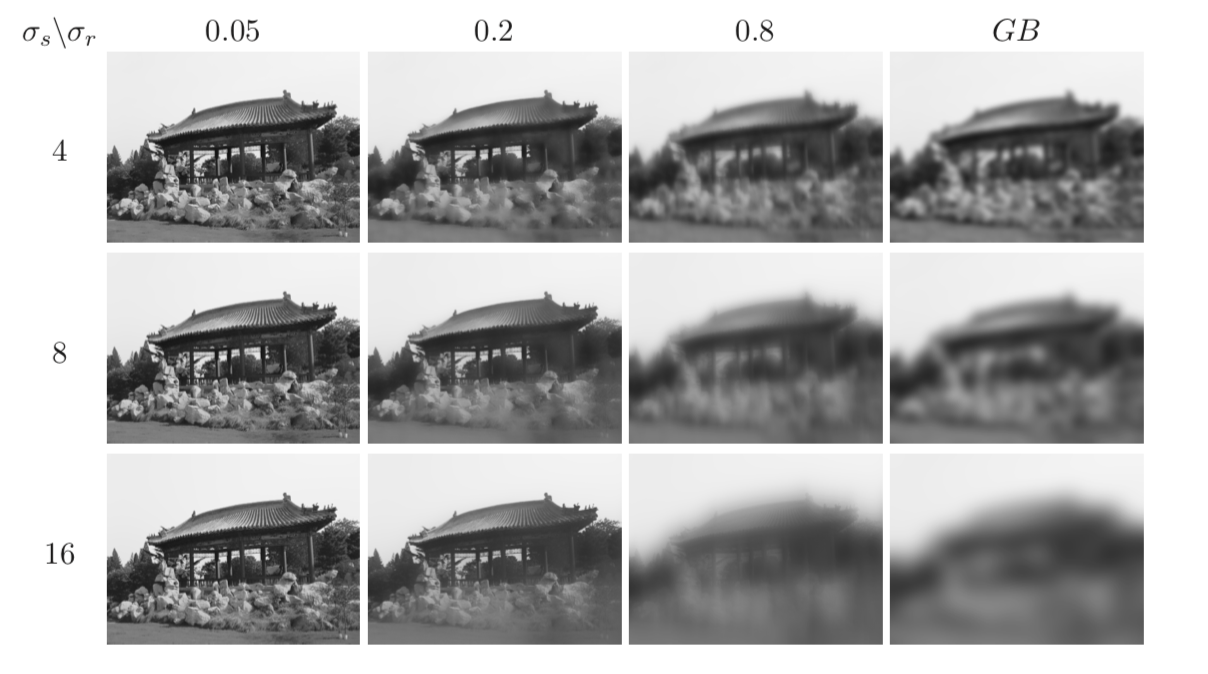
\epsfig{file=kepek/bilateral.png,scale=0.7}
\caption{A $\sigma_r$ és a $\sigma_s$ paraméterek hatása, valamint a Gauss elmosással való összehasonlítás.} 
\label{fig:bilateral}
\end{figure}

\Aref{fig:bilateral1}. ábrán láthatunk egy példát a kétoldalú szűrő elmosására egy bemenetként adott képen, amelyen így az élek megőrzésre kerülnek.

\begin{figure}[h!]
\centering
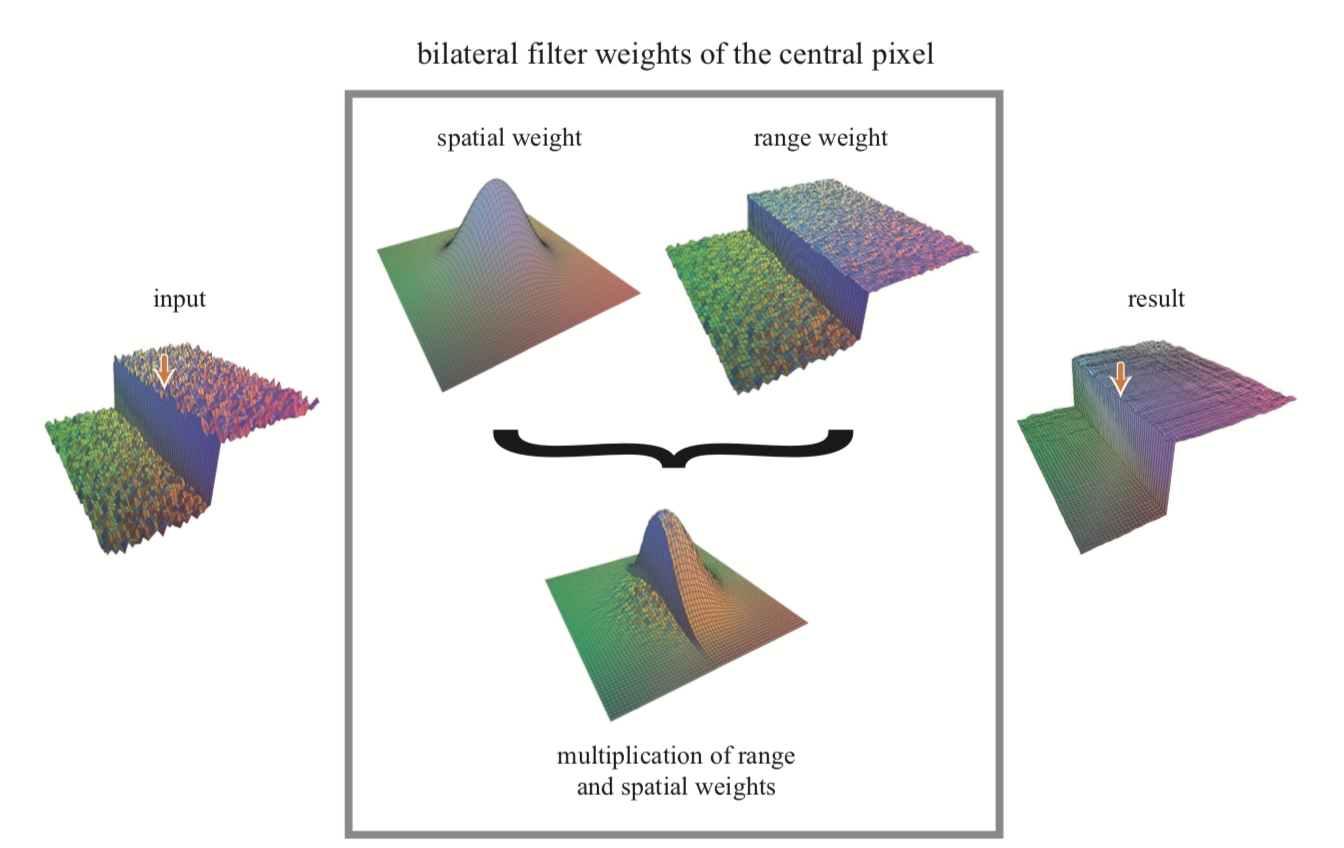
\epsfig{file=kepek/bilateral1.png,scale=0.65}
\caption{A kétoldalú szűrő hatása egy bemeneti képen.} 
\label{fig:bilateral1}
\end{figure}

%wikipédia
%https://people.csail.mit.edu/sparis/bf_course/course_notes.pdf

\newpage

\Section{Éldetektálási módszerek}

Az éldetektálás számos matematikai módszert foglal magába, amelyek olyan pontok azonosítását célozzák meg egy képen, amelyeknél a kép fényereje élesen megváltozik. A kép egy szeletén vizsgálva az intenzitás-profilt jól azonosíthatóak az objektumok határainak megfelelő változások. Az intenzitás-gradiensből következtethetünk az élek helyére és irányára. Jellegzetes élprofilokat láthatunk \aref{fig:elprofilok}. ábrán.

\begin{figure}[h!]
\centering
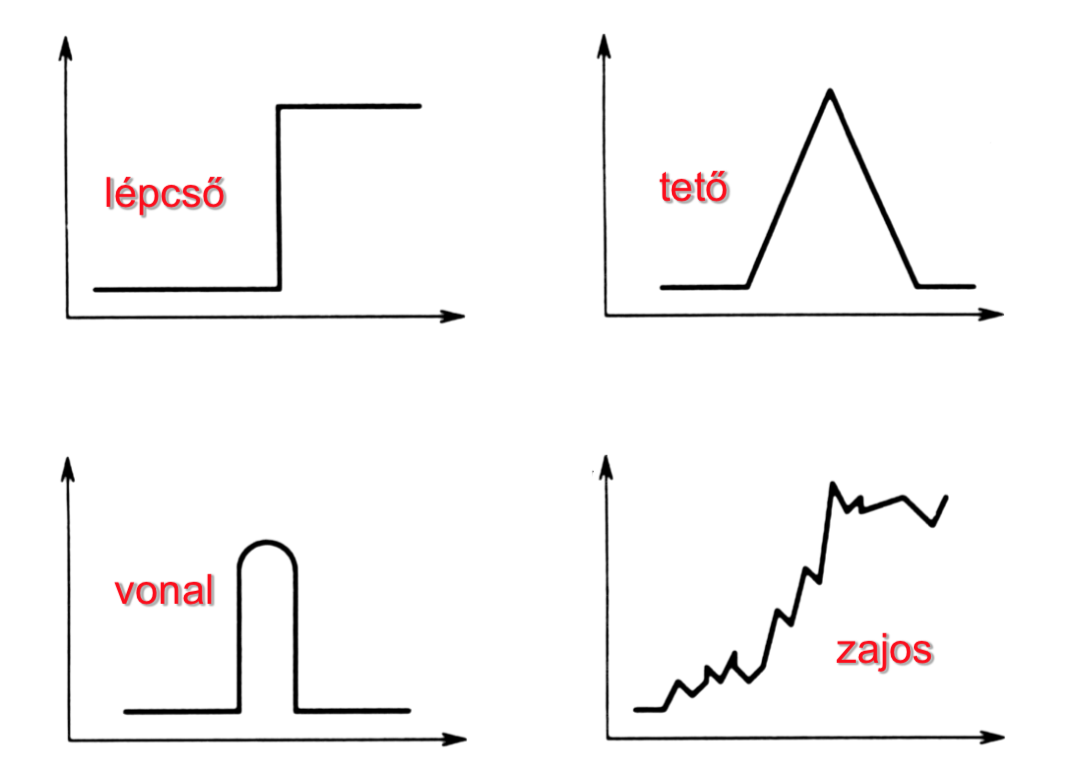
\epsfig{file=kepek/elprofilok.png,scale=0.45}
\caption{Példa tipikus lépcső, tető, vonal és zajos élprofilokra} 
\label{fig:elprofilok}
\end{figure}

A képfüggvény kétváltozós, tehát parciális deriváltakból álló gradiens vektoraink vannak: 
$$
\nabla f =
\left[ \genfrac{}{}{0pt}{}{G_x}{G_y} \right] =
\left[ \frac{\partial f}{\partial x}, \frac{\partial f}{\partial y}  \right]^{T}.$$
A hossza a változás nagyságával egyenlő: 
$$
\left\| \nabla f \right \| =
\sqrt{G_{x}^{2}+G_{y}^{2}} \approx
\left | G_x  \right |+\left | G_y  \right |.
$$
A gradiens a legnagyobb változás irányába mutat: 
$$
\theta = \tan^{-1}\left(\frac{G_y}{G_x}\right).
$$

Digitális képek esetén a pontos, kétváltozós függvényünk nem ismert, ezért a gradiens vektort véges differenciával közelíthetjük:
$$
\frac{\partial f}{\partial x} =
\lim_{\varepsilon \to 0} \left(
\frac{f(x+\varepsilon,y)}{\varepsilon}-\frac{f(x+y)}{\varepsilon}
\right) \approx
\frac{f(x_{n+1}+y)-f(x_n,y)}{\Delta x}.
$$

A gradiens közelítéséhez konvolúciós maszkot is használhatunk.

%Kató tanár úr jegyzet
%wikipédia

\SubSection{Sobel éldetektálás}

% TODO: Roberts éldetektálást is megemlíteni!

A Sobel éldetektáló egy gradiens alapú módszer. Ez elsőrendű deriváltakkal működik. A kép első deriváltját külön számítja az $x$ és $y$ tengelyekhez. A deriváltak csak közelítések (mivel a képek nem folytonosak). Ezek közelítéséhez az alábbi kernelt használják a konvolúcióhoz:
$$\begin{bmatrix}
-1&0  &1 \\ 
-2&0  &2 \\ 
-1&0  &1 
\end{bmatrix},
\qquad
\begin{bmatrix}
-1&-2  &-1 \\ 
0&0  &0 \\ 
1&2  &1 
\end{bmatrix}.
$$
Az első mátrix a vízszintes, a második mátrix a függőleges kernel. A bal oldali kernel megközelíti a deriváltat az $x$ tengely mentén, a jobb oldali pedig az $y$ tengely mentén. Ezen információk felhasználásával számíthatjuk ki az alábbiakat:
\begin{itemize}
\item magnitudója vagy "erőssége" az élnek: $\sqrt{G_{x}^{2}+G_{y}^{2}}$,
\item megközelítő erősség: $ \left\| G_x \right \| + \left\| G_y \right \|$,
\item az él iránya: $arctan\left(\frac{G_y}{G_x}\right)$.
\end{itemize}

%Kató tanár úr jegyzet
%http://aishack.in/tutorials/sobel-laplacian-edge-detectors/

\SubSection{Laplace éldetektálás}

A Laplace éldetektáló csak egy kernelt használ. Másodfoku deriváltakat számol ki egy lépésben. Itt van néhány elterjedt kernel:
$$\begin{bmatrix}
 0 & -1  & 0 \\ 
-1 &  4  &-1 \\ 
 0 & -1  & 0 
\end{bmatrix} 
\qquad
\begin{bmatrix}
-1 & -1 & -1 \\ 
-1 &  8 & -1 \\ 
-1 & -1 & -1 
\end{bmatrix}
$$
Az első mátrix a laplace operátor, a második mátrix a laplace operátor átlókkal.

Használhatjuk akár csak az egyiket, vagy ha jobb közelítést szeretnénk, létrehozhatunk egy 5x5-ös kernelt (aminek a középpontja 24, és minden más -1).

Egy komoly hátrány azonban van, mivel másodfokú deriváltakkal dolgozunk, a laplace éldetektáló rendkívül érzékeny a zajokra. Általában zajcsökkentés szükséges. Néhány fontos további jellemzője:
\begin{itemize}
\item elmosódott élek esetén pontosabb lokalizálást érhetünk el,
\item ebben az esetben csak az élek helyét tudjuk meghatározni, az irányát nem,
\item az operátor nem érzékeny az elforgatásra.
\end{itemize}

%Kató tanár úr jegyzet
%http://aishack.in/tutorials/sobel-laplacian-edge-detectors/

\SubSection{Canny éldetektálás}

Az Canny éldetektálás olyan technika, amely a különböző objektumokból származó hasznos strukturális információkat kivonja, és drasztikusan csökkenti a feldolgozandó adatok mennyiségét. Számos számítógépes képfeldolgozó rendszerben széles körben alkalmazzák. Canny úgy találta, hogy viszonylag hasonlóak a különféle éldetektálás alkalmazására vonatkozó követelmények. Így a követelményeknek megfelelő éldetektáló megoldás számos helyzetben megvalósítható. 
\\ \\
\textbf{Algoritmus:}\\ \\
\indent 1. Gauss simítás\\
\indent 2. A kép intenzitás gradiensének megkeresése\\
\indent 3. Nem-maximumok elhagyása\\
\indent 4. Hiszterézis küszöbölés \\ 

\subsubsection{1. Gauss simítás}

Mivel az éldetektálás eredményeit a képzaj is könnyen befolyásolja, elengedhetetlen a zaj kiszűrése, hogy megelőzze a zaj által okozott hamis detektálást. A kép simítása érdekében Gauss szűrőt alkalmazunk. Ez a lépés enyhén simítja a képet, hogy csökkentse a nyilvánvaló zaj hatását a éldetektálásra.

\subsubsection{2. A kép intenzitás gradiensének megkeresése}

A kép élei különböző irányokban jelennek meg, így a Canny algoritmus négy szűrőt használ a vízszintes, függőleges és átlós élek detektálásához az elmosódott képen. Éldetektáló operátor (például Sobel) az első derivált értékét vízszintes irányban $(G_x)$ és a függőleges irányba $(G_y)$ adja vissza. Ebből meghatározható az él-gradiens és az irány:
$$
G = \sqrt{G_{x}^{2}+G_{y}^{2}},
\quad
\Theta = arctan2\left(\frac{G_y}{G_x}\right).
$$
ahol $G$ a hypot függvény segítségével számítható ki, és az arctan2 az arctangens függvény két argumentummal.

Az élirány-szög négy függőleges, vízszintes és két átlós (0 , 45 , 90  és 135 fokok) függőleges szögek egyikére kerekítve van. Az egyes színsávokba eső élek iránya meghatározott szögértékekre van beállítva.

\subsubsection{3. Nem-maximumok elhagyása:}

A nem-maximumok elhagyása a "vékony" élekre alkalmazzák. A gradiens kiszámítása után a gradiens értékből kivont él még mindig homályos. A 3. kritérium vonatkozásában csak egy pontos válasz lehet az élre. Így a nem-maximumok elhagyása segíthet elhagyni a gradiens értékeket (0-ra állítva), kivéve a lokális maximumokat, amelyek a legerősebb intenzitásérték-változást jelzik. Az algoritmus a következő, minden pixelre a gradiens képen:
\begin{itemize}
\item Hasonlítsa össze az aktuális képpont él-erősségét a pixel él-erősségével, pozitív és negatív gradiens irányba.
\item Ha az aktuális képpont él-erőssége a legnagyobb az azonos irányú maszk más képpontjaihoz képest, az érték megmarad. Ellenkező esetben az érték elhagyásra kerül.
\end{itemize}

Bizonyos implementációkban az algoritmus a folyamatos gradiens irányokat különálló diszkrét irányokba sorolja, majd egy $3 \times 3$ szűrőt rak az előző lépés kimenetre. Minden pixelben elhagyja a középső képpont él-erősségét (az értékét 0-ra állítva), ha nagysága nem nagyobb, mint a két szomszéd nagysága a gradiens irányba.

\subsubsection{4. Hiszterézis küszöbölés:}

Eddig az erős élű képpontokat minden bizonnyal be kell vonni a végső élbe, mivel ezek a kép valódi éleiből származnak.Vannak azonban viták a gyenge élű képpontokról, mivel ezek a pixelek kiválaszthatók az igazi élről, vagy a zaj/színváltozatokról. Pontos eredmény elérése érdekében az utóbbi okok által okozott gyenge éleket el kell távolítani. Általában gyenge él pixeleket okoznak, az igazi élek amikor erős élű pixelekhez kapcsolódnak, amíg a zajok nem kapcsolódnak hozzá. Az élkapcsolat nyomon követéséhez a blob elemzést kell végre hajtani, ami egy gyenge élű pixel és 8-as kapcsolatú szomszédos pixelek figyelembevétele. Mindaddig, amíg van egy erős élű pixel, amely részt vesz a blob elemzésben, a gyenge élű pontot lehet azonosítani, amit meg is kell őrizni.

%Kató tanár úr jegyzet
%wikipédia

\Section{Szegmentálás}

Számítógépes látásmódban a képszegmentálás a digitális kép több szegmensbe való felosztása. A szegmentálás célja egyszerűsíteni és/vagy megváltoztatni a kép reprezentációját ezzel könnyebbé téve a kép elemzését. A kép szegmentálását általában objektumok és határok megtalálásához használják. Pontosabban, a képszegmentálás egy címke hozzárendelését jelenti a kép minden képpontjához úgy, hogy az azonos címkével rendelkező pixelek bizonyos tulajdonságokkal rendelkeznek. A képszegmentáció eredménye olyan szegmensek csoportja, amelyek együttesen fedik le a teljes képet vagy a képből kinyert kontúrt. Valamennyi régióban lévő pixelek hasonlóak bizonyos jellemzők vagy számított tulajdonságok, például szín, intenzitás vagy textúra tekintetében. A szomszédos régiók szignifikánsan különböznek az azonos jellegzetességek tekintetében.

%wikipédia

\SubSection{Mean shift algoritmus}

Mean shift egy eljárás a maximális értékek azonosítására, ahol a sűrűségfüggvény módjait a funkciótól vett diszkrét adat szolgáltatja. Ez egy iteratív módszer, az $x$ kezdeti becslésével kezdünk. Adjuk meg a $K(x_i - x)$ kernel függvényt. Ez a függvény határozza meg a közeli pontok súlyát az átlag újraértékeléséhez. Általában egy Gauss kernelt használunk az aktuális becsléshez képest, $K (x_i - x) = e ^ {- c || x_i - x || ^ 2}$. A $K$ által meghatározott ablak sűrűségének súlyozott átlaga: 
$$
m(x) =
\frac{\sum_{x_i \in N(x)}K(x_i-x)x_i}{\sum_{x_i \in N(x)}K(x_i-x)},
$$
ahol $N(x)$ az $x$ szomszédsága, olyan pontok halmaza, amelyekhez $K(x_ {i}) \neq 0$.

Az $m (x) -x$ különbséget az Fukunaga és a Hostetler átlagos eltolódásának nevezik. Az mean shift algoritmus most beállítja az $x \leftarrow m(x)$ értéket, és megismétli a becslést, amíg $m(x)$-ig konvergál.

\Section{Küszöbölés}

% TODO: Érdemes lehet még az éldetektálás elé rakni!

A küszöbérték a képszegmentálás legegyszerűbb módja. A szürkeárnyalatos képből küszöbérték használatával bináris képek készíthető. Tételezzük fel, hogy az objektum és a háttér eltérő intenzitású, vagyis nagy a kontraszt. Az objektum és a háttér önmagában homogén intenzitású. A küszöbölést így a hisztogram alapján választott megfelelő értékkel el tudjuk végezni (\ref{fig:threshold}. ábra).

Zajos kép esetén nehéz kielégítő köszöbértéket meghatározni, tehát a szegmentálás inhomogén lesz, erre a zajszűrés jelenthet megoldást.

%wikipédia

\begin{figure}[ht]
\centering
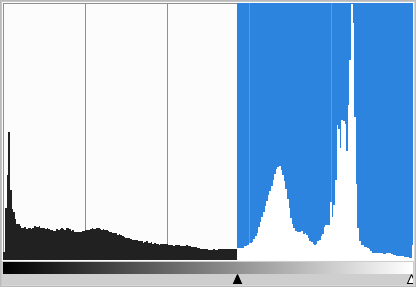
\epsfig{file=kepek/threshold.png,scale=0.65}
\caption{Példa a hisztogram alapján egy megfelelő küszöbérték megválasztására} 
\label{fig:threshold}
\end{figure}

% TODO: Az alábbit még át kell majd kicsit fogalmazni!

\example{Sötét objektum világos háttérben:\\
$f(x,y)$- bemeneti kép;\\
$t(x,y)$- szegmentált kép;\\
$T$=küszöbérték\\
\\
$f(x,y)\leq T$, akkor $t(x,y)=1$, azaz objektum.\\
$f(x,y)> T$, akkor $t(x,y)=0$, azaz háttér.
}\\\\
Léteznek adaptív eljárások, melyek az input képhez automatikusan választják ki az optimális küszöbértéket. Ebből vannak globális és lokális küszöbértéket meghatározó algoritmusok. A globális köszöbölésre alkalmas algoritmusok hisztogramból klaszterezéssel számított értékekel dolgoznak. Ilyen például az Isodata valamint az Otsu algoritmus. A lokális küszöbölés változó értékekkel dolgozik, például egyenletlen megvilágítás. Amennyiben az objektum és a háttér kontrasztja globális küszöbölés után, lokálisan még mindig nagy, akkor alkalmazzuk a lokális küszöbölést, például Niblack algoritmust.

%Kató tanár úr jegyzet
%wikipédia

\SubSection{Izodata algoritmus (Yanni)}

Jól használható, ha az előtér és a háttér körülbelül ugyanannyi képpontból áll. Az algoritmus az alábbi lépésekből áll.
\begin{itemize}
\item[1.] Inicializálás: a hisztogramot kétrészre osztjuk, célszerűen a felezőponton: $T_0$
\item[2.] Kiszámítjuk az objektum valamint a háttér intenzitásának a középértékét: $M_i, m_i$
\item[3.] Az új küszöbérték a két középérték átlaga: $T_i=(M_i+m_i)/2$
\item[4.] Vége ha a küszöbérték már nem változik: $T_k+1=T_k$
\end{itemize}

%Kató tanár úr jegyzet

\SubSection{Otsu algoritmus}

A bemeneti kép $L$ szürkeárnyalatot tartalmaz, a normalizált hisztogram minden $x$ szürkeértékéhez megadja az előfordulási gyakoriságát, vagyis a valószínűségét: $p_x$. Keressük azt a $T$ küszöbszámot, amely maximalizálja az objektum-háttér közötti varianciát.

\textbf{Az előtér/háttér pixelek gyakorisága és középértéke:}

Háttér valószínűsége:
$$
B(T) = \sum\limits_{x=1}\limits^{T}p_x 
$$

Objektum valószínűsége:
$$
1-B(T)=\sum\limits_{x=T+1}\limits^{L}p_x
$$

Legyen $m(T)\equiv \sum\limits_{x=1}\limits^{T}xp_x$, a teljes kép középértéke: $\mu \equiv m(L) = \sum\limits_{x=1}\limits^{L}xp_x$,

Háttér középértéke:
$$
\mu_B =\frac{m(T)}{B(T)}
$$

Objektum középértéke:
$$
\mu_O =\frac{\mu-m(T)}{1-B(T)}\\
$$

\textbf{Az előtér/háttér pixelek szórása:}

$$
\sigma^2_B =
\frac{1}{B(T)}\sum\limits_{x=1}\limits^{T}(x-\mu_B)^2 p_x,
$$
$$
\sigma^2_O =
\frac{1}{1-B(T)}\sum\limits_{x=T+1}\limits^{L}(x-\mu_O)^2 p_x
$$

\textbf{A teljes kép szórása:}
$$
\sigma^2 =
\sum_{x=1}^T(x-\mu)^2 p_x + \sum_{x=T+1}^L(x-\mu)^2 p_x =
\dots =
$$
$$
= B(T)\sigma_B^2+(1-B(T))\sigma_O^2 + (\mu_B-\mu)^2B(T)+(\mu_O-\mu)^2(1-B(T)) \equiv \sigma^2_W(T)+\sigma^2_C(T)
$$
ahol, a $B(T)\sigma_B^2+(1-B(T))\sigma_O^2 = \sigma^2_W(T)$, osztályon belüli varianciától függ és a $(\mu_B-\mu)^2B(T)+(\mu_O-\mu)^2(1-B(T)) = \sigma^2_C(T)$, osztályokközötti varianciától függ. A $\sigma^2$ konstans, és $T$-t úgy kell beállítani, hogy $\sigma_C^2(T)$ a lehető legnagyobb legyen:
$$
\sigma^2_C(T) = \dots = \frac{(\mu(T)-\mu B(T))^2}{B(T)(1-B(T))}
$$
A hisztogram elejéről kezdve nézzük meg minden szürkeértéket, mint lehetséges küszöböt. Kiszámoljuk a $\sigma^2_C(T)$ értéket a $\mu(T)$ és $B(T)$  segítségével, mindaddig növeljök a $T$ értékét, amíg $\sigma^2_C(T)$ kövekszik. Ez az algoritmus feltételezi, hogy $\sigma^2_C(T)$-nek egy maximuma van.

%Kató tanár úr jegyzet

\SubSection{Niblack algoritmus}

Egyetlen küszöb nem elegendő az objektum és a háttér szétválasztásához. Ezért változó köszöbérték $(T(i,j))$ kell, amely követi az intenzitás változásokat:
$$
T(i,j)=\mu(i, j) + k \sigma(i, j)
$$
Az $(i,j)$ adott környezetében, $\mu(i,j)$ a középértéket jelenti, $\sigma(i, j)$ pedig a szórást. A $k$ egy súly, ami megmutatja mennyire vegyük figyelembe a szórást.

Ha $k < 0$, akkor sötét az objektum,
Ha $k > 0$, akkor világos az objektum.

A változó küszöbértékre láthatunk egy szemléltetést \aref{fig:niblack}. ábrán.

\begin{figure}[ht]
\centering
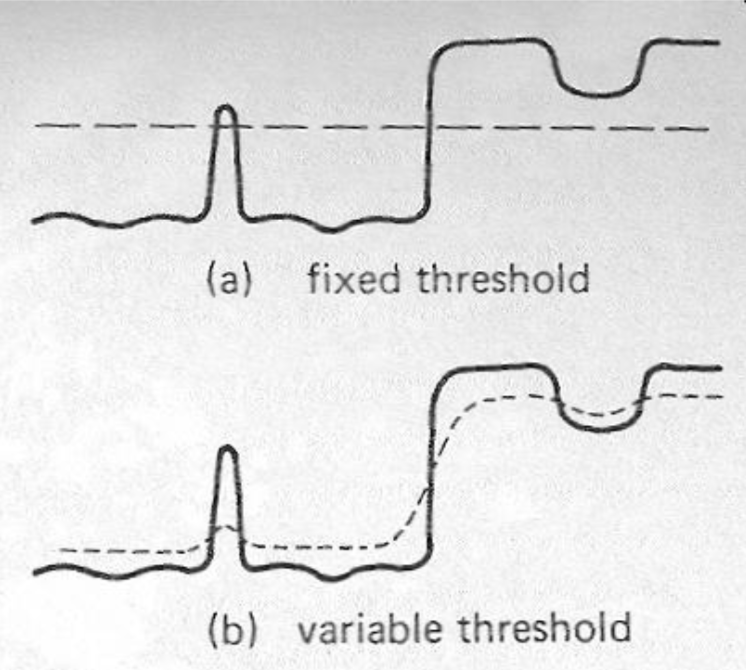
\epsfig{file=kepek/niblack.png,scale=0.65}
\caption{Változó küszöbérték} 
\label{fig:niblack}
\end{figure}

%Kató tanár úr jegyzet
